%% *************************************************************************
%%
%% This is an RIT Space Exploration Standard defining guidelines for content
%% and formatting of project design documents.
%%
%% This document uses IEEEtran.cls, the official IEEE LaTeX class
%% for authors of the Institute of Electrical and Electronics Engineers
%% (IEEE) Transactions journals and conferences.
%%
%% *************************************************************************

%% *************************************************************************
% LaTeX REFERENCES
% ----------------
%   Intro to LaTeX: http://www.rpi.edu/dept/arc/docs/latex/latex-intro.pdf
%   Comprehensive LaTeX symbol list: http://tug.ctan.org/info/symbols/comprehensive/symbols-a4.pdf
%% *************************************************************************

% tell \LaTeX what kind of formatting to use
\documentclass[conference]{IEEEtran} % http://www.ctan.org/pkg/ieeetran
% enable placeholder text generator
\usepackage{blindtext}
% enable toolbox for embedding figures and pictures
\usepackage{graphicx}
\graphicspath{ {img/} }
% enable package for adding a list of variables and constants at the beginning, aka "nomenclature"
\usepackage{nomencl}
% enable package for easily formatting units
\usepackage{siunitx}
% enable package for cross-referencing figures, sections, references etc.
% how to use hyperref: http://www2.washjeff.edu/users/rhigginbottom/latex/resources/lecture09.pdf
\usepackage{hyperref}
% change text encoding to make it more crisp
\usepackage[T1]{fontenc}
% enable conditionals for help text
\usepackage{etoolbox}

\usepackage{booktabs}
\usepackage{hyperref}
\usepackage{tabularx}

% initialize nomenclature package
\makenomenclature{}

% set title. choose something as descriptive and precise as possible. Descriptive > sounding cool. remember this!
\title{Low Cost Nanosatellite for Undergraduate Research}


\author{
  % List the authors of the design document. The Champion should go first.
  % The \$~\$ markers tell \LaTeX{} to treat the text inside to be treated as a math expression. This way you can use operators like \textcaret{} to place characters as superscripts.
  % Some \LaTeX{} templates handle the author block in different ways. For example, the \href{http://www.worldscientific.com/worldscinet/jai}{Journal of Astronomical Instrumentation} requires the authors' addresses and emails to be included as well.
  % The \textbackslash{}thanks command puts the contents inside those brackets in a footnote at the bottom of the first page. Technically speaking, \textbackslash{}thanks is just a specially formatted footnote.
  % IEEE also has a ``long form'' author block for many authors. Check here for more information:
  % \url{https://tex.stackexchange.com/questions/156523/multiple-authors-with-common-affiliations-in-ieeetran-conference-template}
  % Read here for a more advanced options to modifying footnotes in the author block:  \url{http://tex.stackexchange.com/questions/826/symbols-instead-of-numbers-as-footnote-markers}
  %   Here, we use the IEEE long-form author block.
  \IEEEauthorblockN{% This block is for author Names.
    T.J.~Tarazevits\IEEEauthorrefmark{1},
  }
  \IEEEauthorblockA{% This block is for the author Afficliations, aka department and university
    RIT Space Exploration, Rochester Institute of Technology \\ %\\ starts a new line
    Rochester, N.Y. \\
    Email:
    \IEEEauthorrefmark{1}tjt3085@rit.edu,
  }
  %%   Below, we use the short-form author block and basically hack it to suit our needs.
  % Philip~Linden$^{*\dagger}$%
  %   \thanks{$^{*}$Project Champion}%
  %   \thanks{$^{\dagger}$BS/MEng '17, Mechanical Engineering},
  % Austin~Bodzas$^{\ddagger}$%
  %   \thanks{$^{\ddagger}$BS '19, Computer Science},
  % Drew~Walters$^{\S}$%
  %   \thanks{$^{\S}$BS '18, Mechanical Engineering Technology},
  % T.J.~Tarazevits$^{**}$%
  %   \thanks{$^{**}$BS '19, Game Design \& Development}%

  %%   If there are many authors, consider using symbolic, numeric (aka arabic),  alphabet footnotes or a combination thereof.
  %% the recommended order for symbolic footnotes is
  %%   (1) asterisk        *   *
  %%   (2) dagger          †   \dagger
  %%   (3) double dagger   ‡   \ddagger
  %%   (4) section symbol  §   \S
  %%   et cetera. For higher counts, use 2x symbols (1)-(4) (i.e. (5) two asterisks **). Keep cycling through (1)-(4) using 3x, 4x, and so on.
  %%   Note that these symbol codes work in math mode and text mode.
  %%   There are ways to make LaTeX do this for you, but it is more advanced and not entirely necessary, especially for short author lists. Not worth the hassle, in my opinion.
}
% page header for pages other than cover page
\markboth{Low Cost Nano-Satellite}%
{Tarazevits \MakeLowercase{\textit{et al.}}: RIT Space Exploration}

% Initial setup is over, start building the document itself
\begin{document}
\maketitle%
% correct bad hyphenation here, separated by spaces
\hyphenation{explor-ation}

\begin{abstract}
This proposal defines a semester long research project to reproduce the nanosatellite constructed for the \$50Sat project.
Students would be tasked with taking the existing designs and fabricating and assembling components into a complete, functional spacecraft.
This project leverages a low-cost, proven design to build critical skillsets within SPEX as well as producing tangible flight-proven hardware.

      % The abstract is a brief summary of the design document. Typically it includes the purpose of the design document, key goals or objectives, and justifications.
      % Be sure not to confuse the abstract with the introduction.
      % It is easiest to write the abstract after the rest of the paper has been written.
      % That way you can choose key information from the sections that you've already completed and string them together in the abstract.
      % Consider the abstract to be your elevator pitch to anyone reading this design document.
      % What are they reading?
      % What is the goal?
      % Why is it worth my time?
      % The abstract is what will show up in Google results and other search engines, and what people will read when they are deciding what is worth their time and brain power.
\end{abstract}

\label{sec:nomenclature}
\newcommand{\nomunit}[1]{%
\renewcommand{\nomentryend}{\hspace*{\fill}#1}}
\renewcommand{\nompreamble}{
    % If you include mathematical expressions or express variables in the design document, list them with their corresponding definitions here as a list.
    % The two lines below make it look nice when defining units/values to constants.

    % Note that math terms and non-math terms are separated and alphabetized, regardless of the order in which they are defined. (Recall terms \$like this\$ are in the math environment)
    % Read more about advanced nomenclature formatting here:\\
    % \url{https://www.sharelatex.com/learn/Nomenclatures}
  }
\nomenclature{RIT}{Rochester Institute of Technology}
\nomenclature{SPEX}{RIT Space Exploration}
\nomenclature{PDD}{Project Design Document}
\nomenclature{FEA}{Finite Element Analysis}
\nomenclature{PCB}{Printed Circuit Board}
\nomenclature{CSLI}{CubeSat Launch Initiative}
\nomenclature{AMSAT}{Amateur Radio in Space}
% Below are examples of using nomenclature for math symbols and constants or units
% \nomenclature{$\dot{m}$}{Mass flow rate
%   \nomunit{\,\si{\kilo\gram\per\second}}}
% \nomenclature{$c$}{Speed of light
%  \nomunit{\,\SI{2.9979e8}{\meter\per\second}}}
\printnomenclature{}


% HELPFUL HINT: If you get the warning ``Command terminated with space.'' when using a \command try placing ``%'' or ``{}'' immediately following the command.

% The sections included here are required. Additional sections and subsections may be added as necessary.
\section{Introduction}
\label{sec:introduction}
  % The introduction is a place to give background and context before diving into the subject matter.
  % Establish context for the work you are about to propose and the main ideas of the proposition itself.

\IEEEPARstart{\$}{50SAT} (Eagle2) was a collaborative education project undertaken by Morehead State University to produce a nanosatellite at extremely low cost (<\$250).
The satellite was launched via AMSAT in 2013 and continuously operated for over two years.
It was also the first use of the PocketQube form factor for nanosatellites.\cite{PocketQube}
This project would build upon their open source design and implementation of a satellite, to produce a fully functional ground model that replicates all major satellite subsystems and operating modes.


\section{Primary Objective}
\label{sec:primary-obj}
  % At the end of the day, whether the project ``succeeds'' or ``fails'' is judged against the objectives it sought to meet.
  % Note that results that contradict expectations/hypotheses are not failures if the scientific \& engineering methods are followed along the way.
  % Sometimes our expectations are wrong and that can be just as successful as getting data we thought we'd see.
  % What matters are what questions you intend to answer.
  % This is the main purpose or main goal the project hopes to achieve.

The goal is to apply members' knowledge to complete the satellite engineering development process at a small scale using a proven design.
Members will engage in the fabrication, assembly and testing of space-ready hardware and work through the unique challenges presented in such designs.

%\begin{figure}
%  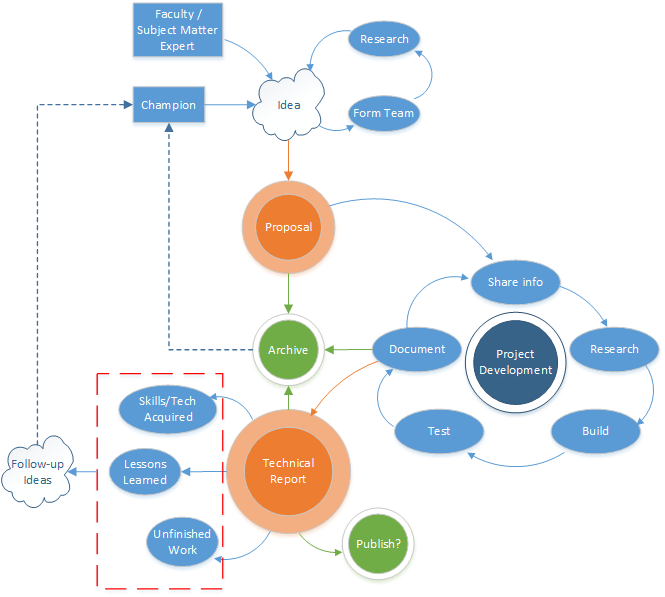
\includegraphics[width=\linewidth]{figs/project-life-cycle.png}
%  \caption{A PDD is the first piece of documentation to be archived in the project life cycle. Since the life cycle can be iterative, a new design document may also refer to one or more previous SPPs.}
%\label{fig:lifecycle}
%\end{figure}

% \section{Secondary Objectives}
% \label{sec:secondary-obj}
% Secondary Objectives are lower priority or bonus objectives that are significant but not the main focus of the project. This template does not have secondary objectives.

\section{Benefit to SPEX}
\label{sec:benefit}
% One of the core values of SPEX is to provide opportunities for academic and professional growth for its members,
% and to challenge them with interesting projects.
% In this section, explain how the project would benefit SPEX members as students,
% space enthusiasts, and young professionals.

This project will have several key benefits to SPEX in the near and long-term.
This project will create a practical astronautical engineering skillset among SPEX members, and will provide opportunities when engaging with employers to showcase the application of member skills.

% Below I have used subsections to identify key ideas in this section. These particular subsections are not required as part of the SPEX Standard, but serve as an example of using subsections in a text.

\subsection{Technical Skill Development}
\label{subsec:technicalSkills}
This multidisciplinary project will require members to learn and apply technical skills to achieve success.
Skills learned during the course of this project can be applied to many other SPEX activities as well as leveraged for future job opportunities.
The scope of this project is ideally suited for undergraduates to undergo the whole development process and gain experience with fabrication and testing techniques on actual space-rated designs.


\subsection{Published Content}
\label{subsec:PublishedContent}
The end goal of this project is to replicate the results of the original \$50SAT hardware design.
The team should produce a report describing the work done, any modifications to the original design, as well as any unforseen technical challenges encountered during the development process.
This will be used internally to inform future projects relating to nanosatellites.

Images, videos, and test result data will be available to share via the SPEX website.

\section{Implementation}
\label{sec:implementation}
  % What path do you anticipate the project to take?
The project will begin by evaluating the existing designs generated by the \$50SAT team, followed by fabrication of subcomponents, and then a final assembly and testing phase.

\subsection{Deliverables}
\label{subsec:deliverables}
  % When all is said and done, what will you have to show for it?
  % Examples: Hardware, software, poster, ImagineRIT demo, presentations, technical papers...

The primary deliverable will be the finished, functioning nanosatellite unit.
In addition, the team should include a report consisting of the following sections:
\begin{itemize}
  \item A summary of the development process, including any unforseen issues that arose during development and detailed explanations on how they were addressed.
  \item Details on any changes to the original design and well as the reasoning for those changes
  \item Detailed operations guide for handling and operating the satellite
  \item Where possible, instruction guides for assembly of key components and subsystems that future teams could leverage.
  \item Test procedures and results for key areas including radio performance, thermal and structural tolerance, and software qualifications
\end{itemize}
The published designs also include an arduino-based radio receiver station. The team could develop this component as well, or preferably, leverage other teams and their projects to satisfy this requirement.
Finally, the team will need to generate a presentation poster that could be used at ImagineRIT or other public SPEX events to highlight the project.

\subsection{Milestones}
\label{subsec:milestones}
  % Be as detailed as you can, but it's okay if there are unknowns.
  % At the very least, specify how many semester you expect the project to take until it reaches completion.
If this project is conducted over a semester timeline, the team will need to expediently cover the required areas defined below.

This project will take place over three technical domains: electrical, mechanical, and software.

For the electrical systems, the team will need to review the existing PCB designs, primarily to determine whether it is feasible to manufacture and populate them on campus.
Also the team will need to determine if all components required are still available, and if not, find suitable replacements and make the necessary design changes.
PCB assembly will be the system with the longest lead time and should be prioritized first to ensure no bottlenecks on the critical path.
Once assembled, each will need to be tested, and integrated within the system structure.

For the mechanical systems, the team should evaluate the feasibility of manufacturing the frame on-campus.
Any tweaks to the internal structure and placement of internal components should be locked down as early as possible.
The mechanical team will also be responsible for testing the frame and whole assembly for verification against thermal and vibration requirements.

For the onboard software, the team should review the existing code, and try to demonstrate functionality on similar hardware to prevent dependency on the electrical team.
Once the primary electronics are ready, the software should be tested for functionality on the system hardware.
\autoref{tab:timeline} shows a preliminary timeline for the project.

\begin{table}
  \caption{Estimated Timeline}
  \centering
  \begin{tabularx}{\columnwidth}{@{}cXl@{}} \toprule
    Phase & Task & Duration \\ \midrule
    1 & Review existing \$50SAT designs and materials & 2 weeks or less \\
    2 & Subsystem development & 6 weeks \\
      & Order PCB design and/or assembly & 6 weeks \\
      & Review changes to mechanical strucuture and order materials & 2 weeks or less \\
      & Testing of individual subsystems & 2 weeks \\
    3 & System Assembly & 1 week  \\
    4 & System testing & 2 weeks  \\
    5 & Generate documentation and delivery to SPEX & 1 week  \\
    \bottomrule
  \end{tabularx}
\label{tab:timeline}
\end{table}

Schedule slip is tolerable, since there are few external considerations within the fall semester, e.g.\ a competition or public display event.
\section{Externalities}
  % Things not directly related to the work or outcomes, but related to the project as a whole.
\subsection{Prerequisite Skills}
  % Which skills do team members need to have before work can start (not including skills that will be learned ``on the job'')?
Firstly, this project requires technical skillsets across multiple disciplines in order to be a success.
The members that make up this project team will need applicable skills to their working domain and general awareness of the space environment and constraints.

Electrical team members should have basic soldering skills, with at least one member familiar with PCB design and layout.
Each board is flight-proven, but should be verified by members with applciable electrical engineering knowledge.
Assembly of those boards will require SMT mounting skills.
Also, prior experience working with solar cells is a plus.

The frame and interal structure of the satellite requires mechanical engineering design and fabrication skills.
Mechanical team members should be able to machine required components and finish final assembly.
At least one member should have the ability to run structural and vibrational FEA on the system designs.
At least one member should have the ability to run thermal FEA.\@

The software is written in Basic for the PICAXE processor, but will need computer science skillsets to validate the codebase and make any necessary modifications.
Software team members should be familiar with C/C++ and object-oriented programming.
Experience with hardware interfaces such as I2C/SPI is a plus.

The ground station and radio communication will require knowledge of physical radio properties and various radio modulation techniques.
Other astronautical engineering skillsets may be required, dependent on unforseen technical challenges.


\subsection{Funding Requirements}
  % Estimate costs that would be needed to meet objectives.
This project should not exceed \$500 in total costs incurred.

The original \$50SAT project cost less than \$250 in raw materials so this project should be within a similar range.
Potential sources for cost inflation include going with an external assembler of the PCBs, and unforseen changes in the design.

An Interactive Learning Grant (ILG) should be able to cover the total expected cost of the project, however it would be prudent to have backup funding available in case of budget overruns.
The project team should give the SPEX administration a preliminary BoM and cost estimate once their initial review of the designs are complete, to aid in securing funding.

\subsection{Faculty Support}
  % Identify faculty that will be involved (or would need to be involved) to meet objectives.
  % Note that if a professor is the Principal Investigator (P.I.) for a project, there still needs to be a student as the SPEX Project Champion.
Faculty support is recommended for teams pursing this project.
The electrical subsystems would most significantly benefit from faculty advisement to review the final assembled board and solar panel assemblies.
Also the radio and antennas system testing would benefit from SPEX advisor expertise and oversight.

\subsection{Long-Term Vision}
\label{sec:vision}
This project would result in SPEX's first functional, space-rated hardware project.

Future teams could utilize the same low cost design philosphy while pushing the boundaries in one or more subsystems over time to create a more compelling spacecraft.
The skils learned from this project would mitigate the risk of future projects with increased technical complexity.

If this project was iterated on, hardware developments and experience gained from these projects could be applied to a CubeSat or other nanosatellite that would actually fly in space, through a launch partnership like CSLI.\@

\section*{Acknowledgements}
The author would like to thank Professor Bob Twiggs at Morehead State University and the rest of the \$50SAT team for publishing open source design for the mission, allowing similar student teams to work on flight-proven hardware.

\bibliography{SPEX50SAT}
\onecolumn
\appendices{}
\section{\$50SAT Reference Images}
\begin{figure}[h]
 \centering
 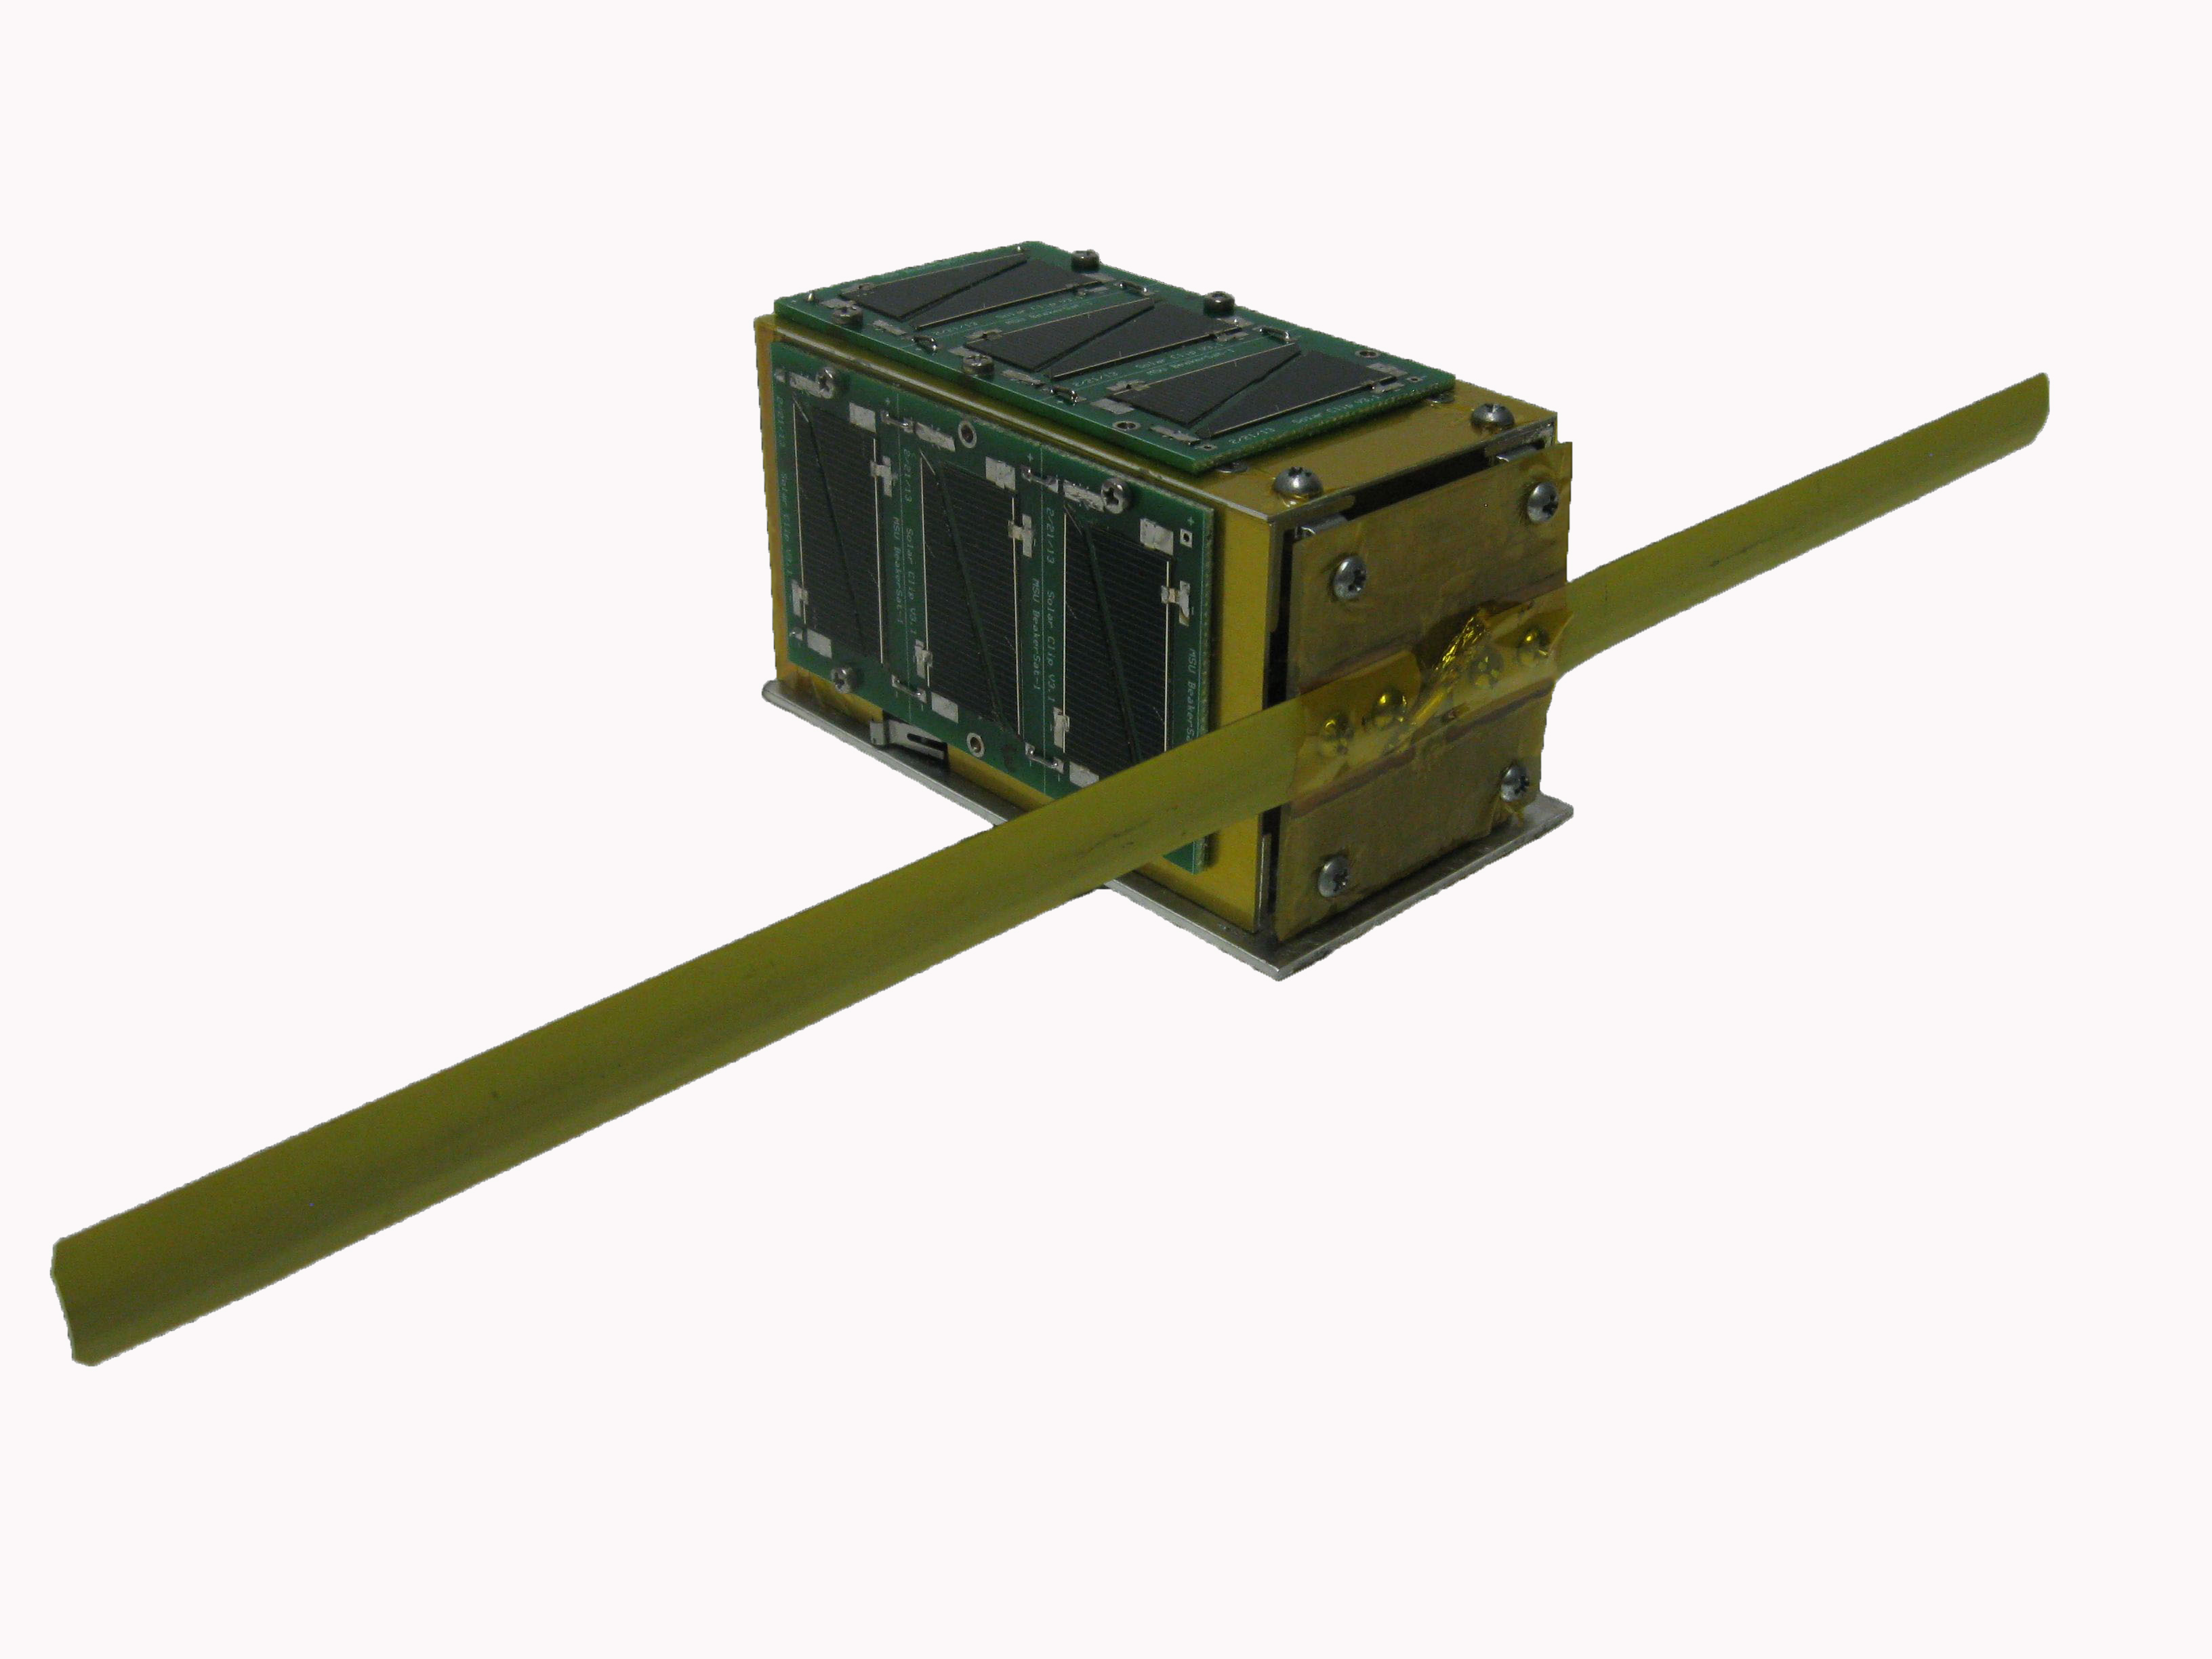
\includegraphics[width=12cm, height=9cm]{50sat_model.jpg}
 \caption{3D rendering of the complete \$50SAT satellite.}
\end{figure}

\begin{figure}[h]
 \centering
 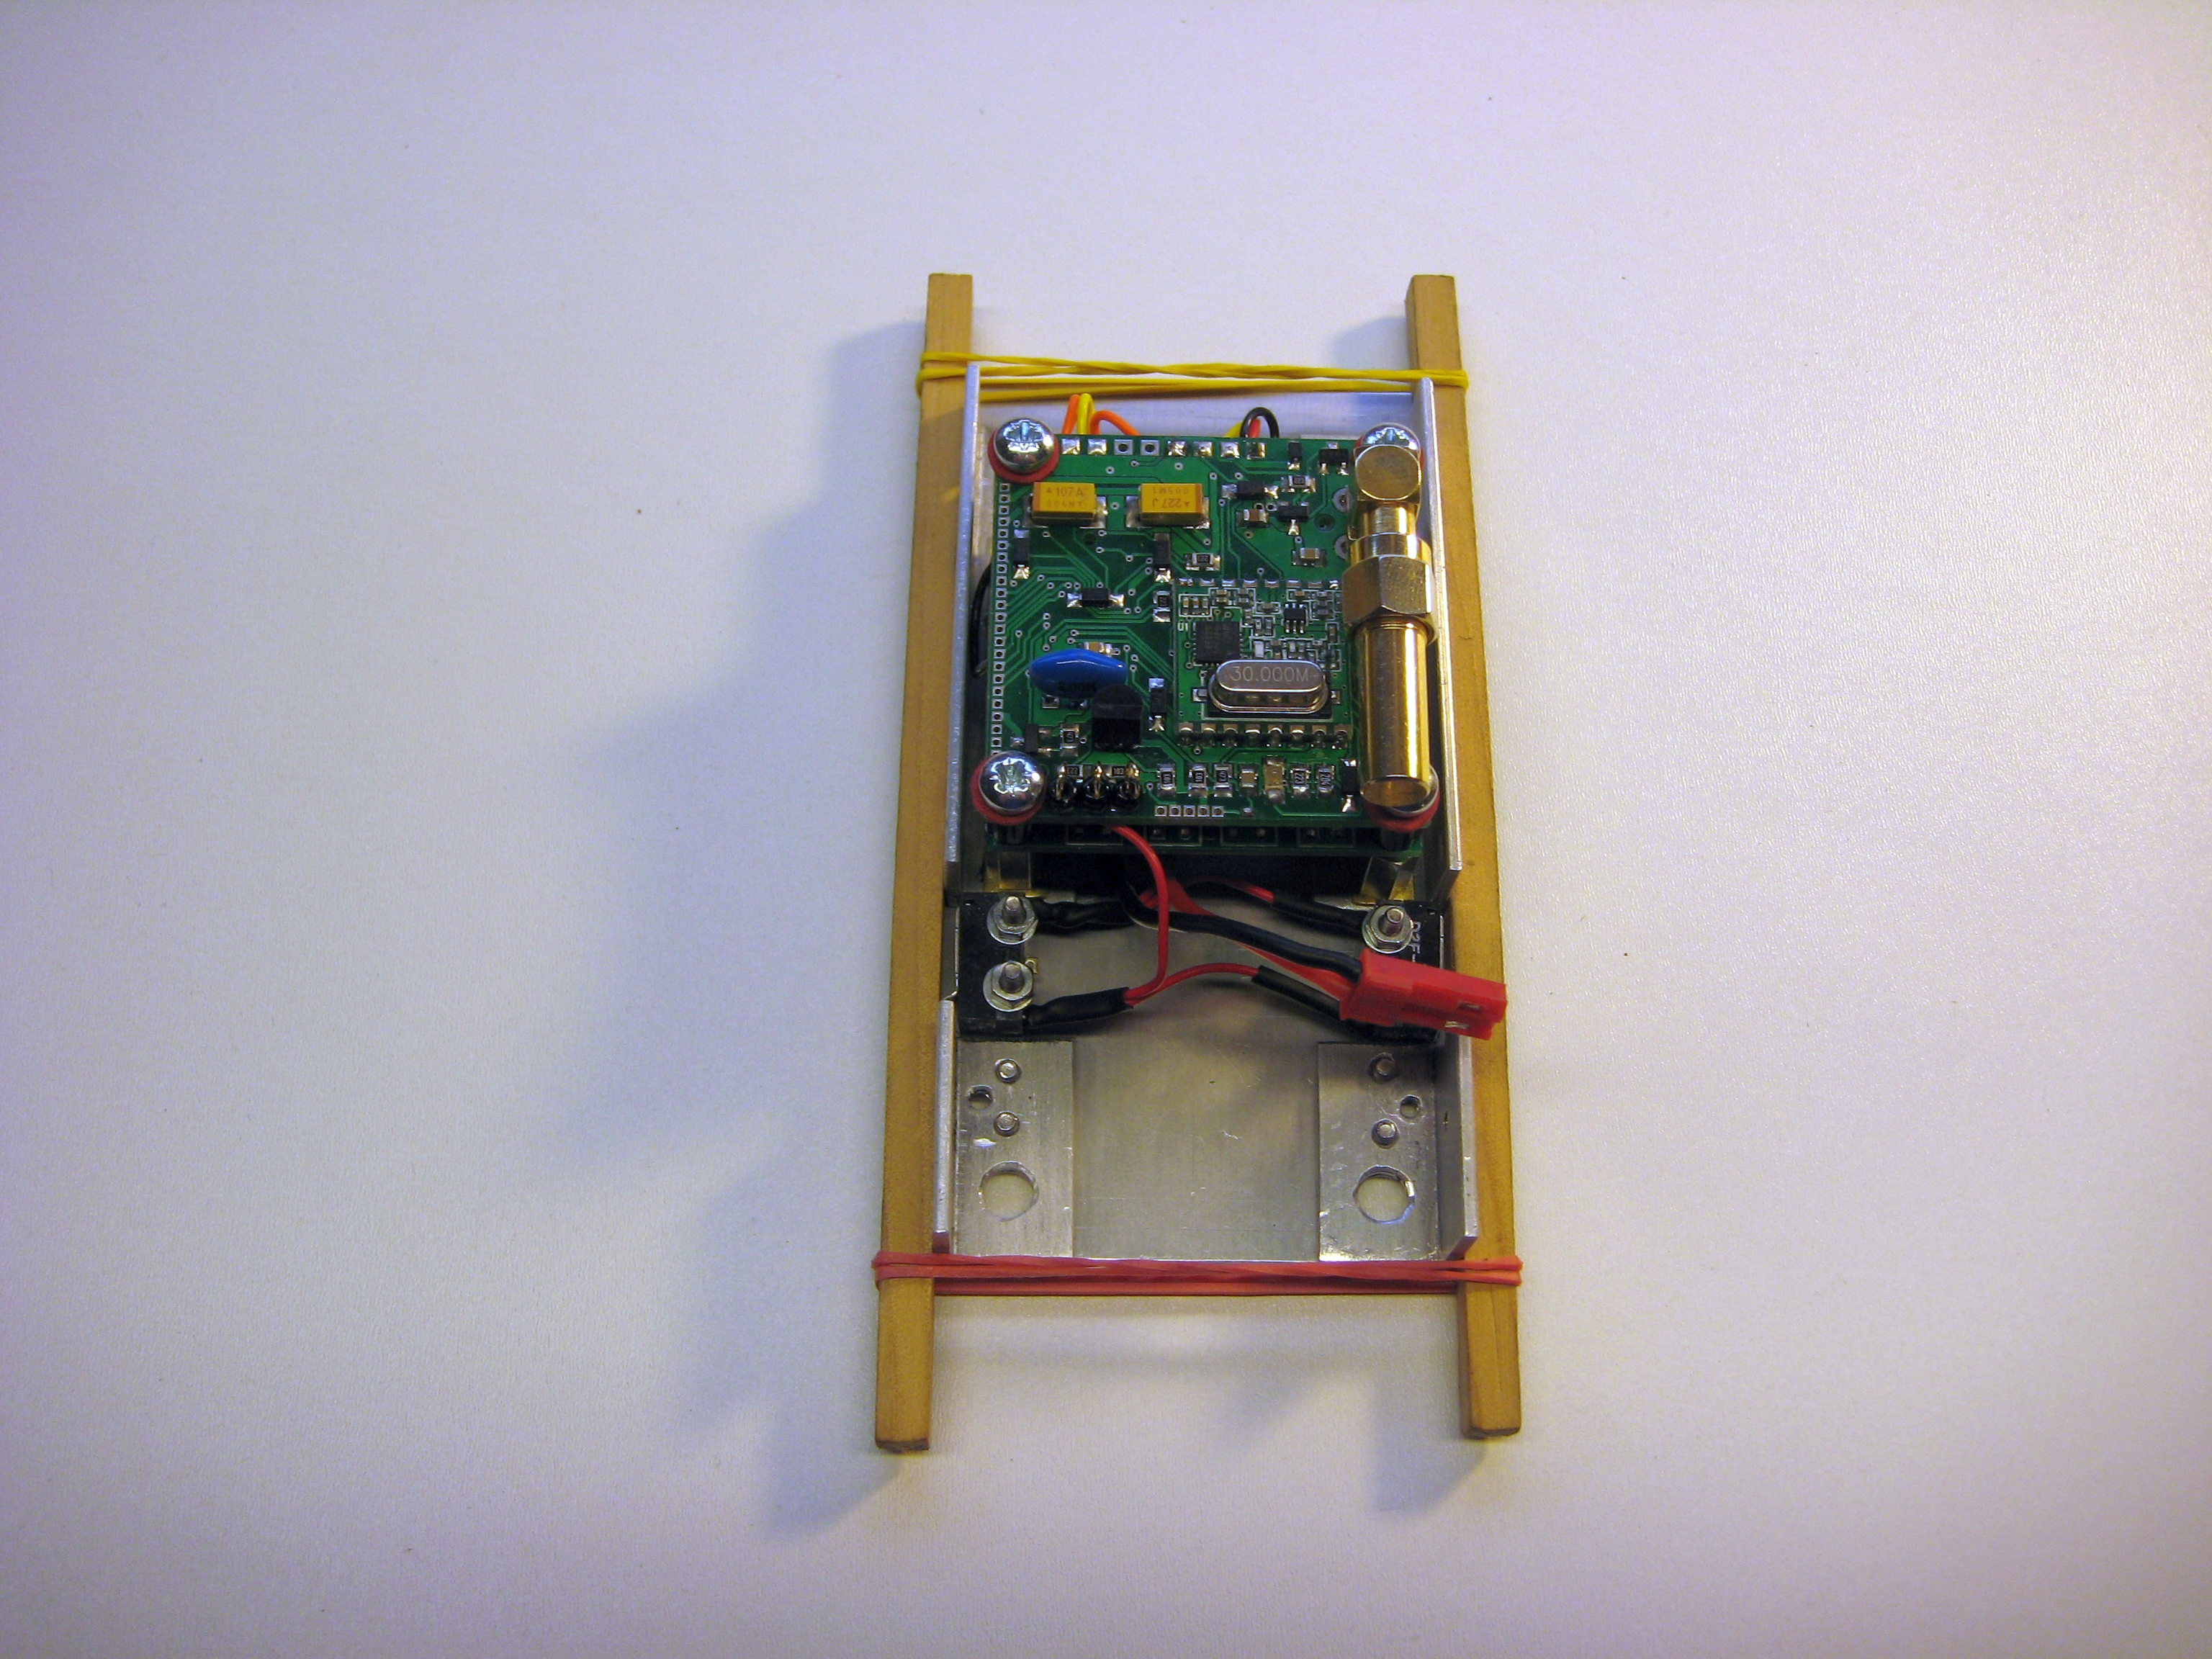
\includegraphics[width=12cm, height=9cm]{internal_pcbs.jpg}
 \caption{View of the layout of the internal electronics.}
\end{figure}

\end{document}
